\textbf{Цель работы:} исследовать явление проникновение переменного магнитного поля в медном полом цилиндрe.\\\indent
\textbf{Оборудование:} генератор сигналов; соленоид, намотанный на полый цилиндрический каркас; медный экран в виде полого цилиндра; измерительная катушка; амперметр; вольтметр; двухканальный осциллограф; RLC-метр.

\section*{Теоретические сведения}
\subsection*{Магнитное поле внутри и вне экрана}
\begin{wrapfigure}{l}{0.23\linewidth}
    \centering
    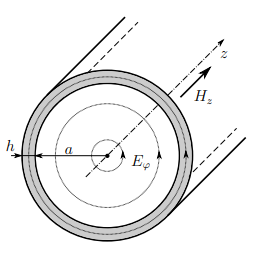
\includegraphics[width=4cm]{images/theory.png}
    \caption{Поле в тонкостенном цилиндре}
\end{wrapfigure}
\indent Пусть цилиндр достаточно длинный, чтобы в нем можно было пренебречь краевыми эффектами и считать магнитное поле $H$ внутри однородным, направленным вдоль оси OZ, а вихривое поле $E$ будет препендикулярно радиусу. $H$ и $E$ - величины колеблющиеся по гармоническому закону с частотой $\omega$, задаваемой частотой колебаний тока в соленоиде: $H_z = H(r)e^{i\omega t}$, $E_{\varphi} = E(r)e^{i\omega t}$.\\\indent
Пусть полый цилиндр имеет радиус $a$ и толщину стенок $h \ll a$. Тогда поле в цилиндре описывается уравнением:
\begin{equation}
    \frac{d^2 H}{d x^2} = i\omega\sigma\mu_0 H
\end{equation}
Граничные условия для $H$: 
\begin{align}
    H(0) = H_0, \hspace{0.5cm}  H(h) = H_1
\end{align}
Рeшение (1) ищем в виде $H(x) = Ae^{\alpha x} + Be^{-\alpha x}$, где $\alpha = \sqrt{i\omega \sigma \mu_0} = \frac{1 + i}{\delta} = \frac{\sqrt{2}}{\delta}e^{i\pi/4}$.\\
Решая уравнение (1) при начальных условиях (2) получаем:
\begin{align}
    \delta &= \sqrt{\frac{2}{\omega \sigma \mu_0}}\label{eq:delta}\\ 
    H_1 &= \frac{H_0}{\ch (\alpha h) + \frac{1}{2}\alpha a\sh(\alpha h)}
\end{align}
Рассмотрим предельные случаи:\\ 
\indent \textbf{1. При малых частотах} $\delta \gg h$ и тогда 
\begin{equation}
    H_1 \approx \frac{H_0}{1 + i\frac{a h}{\delta}}
\end{equation}
И тогда отношение модулей амплитуд:
\begin{equation}
    \frac{|H_1|}{|H_0|} = \frac{1}{\sqrt{1 + \left (\frac{a h}{\delta^2}\right )^2}} = \frac{1}{\sqrt{1 + \frac{1}{4}(a h \sigma \mu_0 \omega)^2}} \label{eq::Hrelation}
\end{equation}
А колебания $H_1$ отстают по фазе от $H_0$ на угол $\psi$:
\begin{equation}
    tg\psi = \frac{a h}{\delta^2} \label{eq:tgpsi}
\end{equation}

\indent \textbf{2. При достаточно больших частотах} $\delta \ll h$ и отношение амплитуд выражается как:
\begin{equation}
    \frac{H_1}{H_0} = \frac{4}{\alpha a}e^{-\alpha h} = \frac{2\sqrt{2}\delta}{a}e^{-\frac{h}{\delta}}e^{-i\left( \frac{\pi}{4} + \frac{h}{\delta}\right)}
\end{equation}
Отсюда видно, что поле внутри цилиндра по модулю в $\frac{2\sqrt{2}\delta}{a}e^{-\frac{h}{\delta}}$ раз меньше, чем снаружи и в запаздывает по фазе на:
\begin{equation}
    \psi = \frac{\pi}{4} + \frac{h}{\delta} = \frac{\pi}{4} + h\sqrt{\frac{\omega\sigma\mu_0}{2}} \label{eq:psi}
\end{equation}

\subsection*{Влияние скин-эффектра на индуктивность катушки}
\indent На высоких частотах магнитное поле не проникает за экран, поэтому суммарный магнитный поток, пронизывающий
катушку, уменьшается, и, соответственно, уменьшается и индуктивность. При низких частотах, когда толщина скин-слоя $\delta$ больше толщины медного экрана $h$, магнитное поле
проникает внутрь катушки, однако его амплитуда падает (по формуле (6)) и возникает
разность фаз между колебаниями поля за экраном и перед ним (по формуле (7)). Из-за
чего также изменяется магнитный поток, а следовательно – и индуктивность.
\begin{equation}
    \Phi = \Phi_{out} + \Phi_{in} = H_0S_0 + H_1S_1 = LI
\end{equation}
При этом $L_{min} = \frac{\Phi_{out}}{I}$ и не зависит от частоты. 
Выразим поток магнитного поля сквозь внутреннюю область $\Phi_{in}$ через поток сквозь
внешнюю $\Phi_{out}$ при произвольном переменном токе $I$:
\begin{equation}
    \Phi_{in} = H_1S_1 = \frac{H_1S_1}{H_0S_0}\Phi_{out} = \frac{\Phi_{out}}{n}\frac{S_1}{S_0}
\end{equation}
где $n$ - коэффициент, характеризующий ослабление поля за экраном:
\begin{equation}
    n = \frac{H_0}{H_1} = \frac{|H_0|}{|H_1|}\frac{1}{\cos\psi}
\end{equation}
Максимальная индуктивность катушки достигается при $H_0 = H_1$:
\begin{equation}
    \Phi_{max} = H_0(S_0 + S_1) = L_{max}I_m \text{, где} \hspace{0.3cm} H_0S_0 = L_{min}I_m
\end{equation}
Тогда получаем:
\begin{align}
    \frac{S_1}{S_0} &= \frac{L_{max} - L_{min}}{L_{min}}\\
    L &= L_min + \frac{L_{max} - L_{min}}{n}\\ 
    \frac{L_{max} - L}{L - L_{min}} &= (\pi a h \mu_0 \sigma \nu)^2
\end{align}

\section*{Экспериментальная установка}
\indent Переменное магнитное поле создается с помощью соленоида 1, намотанного на цилиндрический каркас 2, который подключается к генератору сигналов. Внутри каркаса расположен медный экран 3 в виде полого
цилиндра.
\\\indent Действующее значение переменного тока в цепи соленоида измеряется цифровым амперметром «А». Действующее значение переменного напряжения на измерительной катушке 4 измеряется цифровым вольтметром «V».
\\\indent Для измерения сдвига фаз между током в цепи соленоида и напряжением на измерительной катушке используется двухканальный осциллограф. На один канал осциллографа подается напряжение с измерительной катушки, а на другой —
напряжение с резистора R, которое пропорционально току в цепи соленоида.
\begin{figure}[h!]
    \centering
    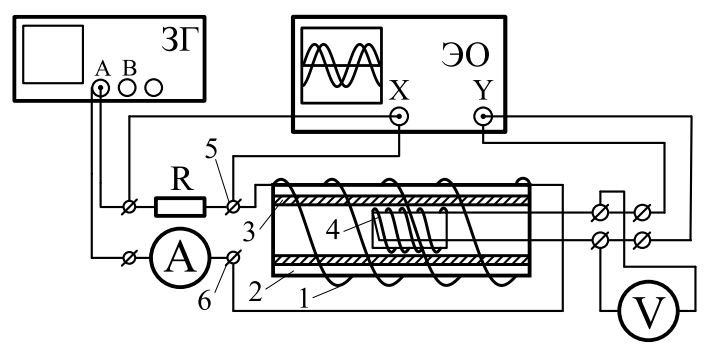
\includegraphics[width=12cm]{images/setup.png}
    \caption{Схема экспериментальной установки}
\end{figure}
\indent С помощью вольтметра V измеряется действующее значение ЭДС индукции, которая возникает в измерительной катушке, находящейся в переменном магнитном поле $H_1e^{i\omega t}$. Комплексная амплитуда ЭДС индукции в измерительной катушке равна:
\begin{equation}
    \bar{U} = -SN\frac{dB_1(t)}{dt} = -i\omega\mu_0 S N H_1e^{i\omega t}
\end{equation}
Показания вольтметра:
\begin{equation}
    U = \frac{S N\omega}{\sqrt{2}}\mu_0|H_1|\hspace{0.2cm} \Rightarrow \hspace{0.2cm}|H_1| \propto \frac{U}{\nu}
\end{equation}
При этом поле вне экрана $|H_0|$ пропорционально току в цепи соленоида. Поэтому
\begin{equation}
    \frac{|H_1|}{|H_0|} = const\cdot\frac{U}{\nu I}
\end{equation}
\section*{Экспериментальные данные и обработка результатов}
\subsection*{Измерения при низких частотах}
\begin{wraptable}{l}{0.38\linewidth}
    \centering
    \begin{tabular}{|c|c|c|c|}
        \hline
        $a$, мм & $h$, мм & $\nu_h$, кГц & $\sigma$, См/м\\\hline
        45 & 1.5 & 2.3 & $5\cdot 10^7$\\\hline
    \end{tabular}
    \caption{Параметры установки}
\end{wraptable}
\indent В области низких частот (от $\sim 0.01\nu_h$ до $0.05\nu_h$) измерили силу тока в цепи и напряжение. Получили зависимость $\xi = \frac{U}{I\nu}$ от частоты $\nu$. Cогласно формуле (19) график в координатах $1/\xi^2 = f(\nu^2)$ должен быть линейным, что можно наблюдать на \ref{fig:plot1}.
\begin{figure}[h!]
    \begin{minipage}{0.5\linewidth}
        \centering
        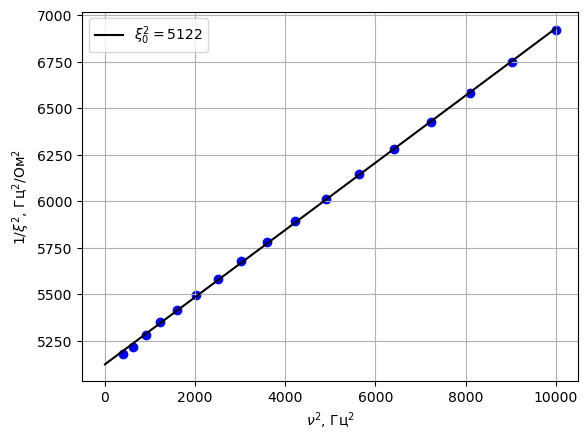
\includegraphics[width=10cm]{images/plot1.png}
        \captionof{figure}{Гарфик $1/\xi^2 = f(\nu^2)$}\label{fig:plot1}
    \end{minipage}
    \begin{minipage}{0.6\linewidth}
        \centering
        \begin{tabular}{|c|c|c|}
            \hline
            $\nu$, Гц & $I$, мА & $U$, мВ\\\hline
            20 & 447.66 $\pm$ 0.05 & 124.4 $\pm$ 0.1\\\hline
            25 & 446.68 $\pm$ 0.05 & 154.6 $\pm$ 0.1\\\hline
            30 & 445.03 $\pm$ 0.05 & 183.7 $\pm$ 0.1\\\hline
            35 & 442.96 $\pm$ 0.05 & 212.0 $\pm$ 0.1\\\hline
            40 & 440.57 $\pm$ 0.05 & 239.5 $\pm$ 0.1\\\hline
            45 & 437.94 $\pm$ 0.05 & 265.9 $\pm$ 0.1\\\hline
            50 & 435.08 $\pm$ 0.05 & 291.2 $\pm$ 0.1\\\hline
            55 & 432.14 $\pm$ 0.05 & 315.4 $\pm$ 0.1\\\hline
            60 & 428.73 $\pm$ 0.05 & 338.4 $\pm$ 0.1\\\hline
            65 & 425.51 $\pm$ 0.05 & 360.3 $\pm$ 0.1\\\hline
            70 & 422.23 $\pm$ 0.05 & 381.2 $\pm$ 0.1\\\hline
            75 & 418.96 $\pm$ 0.05 & 400.9 $\pm$ 0.1\\\hline
            80 & 415.64 $\pm$ 0.05 & 419.6 $\pm$ 0.1\\\hline
            85 & 412.34 $\pm$ 0.05 & 437.2 $\pm$ 0.1\\\hline
            90 & 409.08 $\pm$ 0.05 & 453.8 $\pm$ 0.1\\\hline
            95 & 405.87 $\pm$ 0.05 & 469.4 $\pm$ 0.1\\\hline
            100& 402.71 $\pm$ 0.05 & 484.1 $\pm$ 0.1\\\hline
        \end{tabular}
        \captionof{table}{Показания вольтметра и амперметра при низких частотах от $0.01\nu_h$ до $0.05\nu_h$}
    \end{minipage}
\end{figure}
\\\\
Экстраполируя зависимость к точке $\nu = 0$, соответствующей $|H_1|/|H_0| = 1$, определяем $\xi_0 = 71.69\pm0.03$ Гц/Ом. По формуле \ref{eq::Hrelation} определяем проводимость меди $\sigma = (4.390 \pm 0.002)\cdot10^7$ См/м.

\subsection*{Измерения при средних и высоких частотах}
\indent Теперь повторим измерения, но для средних (от $0.05\nu_h$ до $0.1\nu_h$) и высоких (от $0.5\nu_h$ до $15\nu_h$) частот.\\\indent По грфику $tg\psi(\nu)$, опираясь на формулы \ref{eq:delta} и \ref{eq:tgpsi} определим проводимость материала экрана $\sigma = (5\pm 1.5)\cdot 10^7$ См/м.\\\indent
По грфику $\psi - \pi/4 = f(\sqrt{\nu})$, опираясь на формулy \ref{eq:psi} определим проводимость материала экрана $\sigma = (4.9\pm 0.5)\cdot 10^7$ См/м.
\newpage
\begin{table}[h!]
    \centering
    \begin{tabular}{|c|c|c|c|}
        \hline
        $\nu$, Гц & $I$, мА & $U$, мВ & $\psi$, рад\\\hline
        100 & 400.57 $\pm$ 0.05 & 482.4 $\pm$ 0.1 & 0.56 $\pm$  0.13\\\hline
        120 & 388.75 $\pm$ 0.05 & 532.8 $\pm$ 0.1 & 0.56 $\pm$  0.13\\\hline
        140 & 378.32 $\pm$ 0.05 & 571.9 $\pm$ 0.1 & 0.69 $\pm$  0.13\\\hline
        160 & 369.26 $\pm$ 0.05 & 602.1 $\pm$ 0.1 & 0.75 $\pm$  0.13\\\hline
        180 & 361.48 $\pm$ 0.05 & 625.5 $\pm$ 0.1 & 0.81 $\pm$  0.13\\\hline
        200 & 354.82 $\pm$ 0.05 & 643.7 $\pm$ 0.1 & 0.87 $\pm$  0.13\\\hline
        300 & 332.83 $\pm$ 0.05 & 689.8 $\pm$ 0.1 & 1.06 $\pm$  0.13\\\hline
        400 & 320.33 $\pm$ 0.05 & 702.4 $\pm$ 0.1 & 1.19 $\pm$  0.13\\\hline
        500 & 311.3  $\pm$ 0.05 & 702.1 $\pm$ 0.1 & 1.25 $\pm$  0.13\\\hline
        600 & 303.54 $\pm$ 0.05 & 695.5 $\pm$ 0.1 & 1.31 $\pm$  0.13\\\hline
        700 & 296.25 $\pm$ 0.05 & 685.4 $\pm$ 0.1 & 1.38 $\pm$  0.13\\\hline
        800 & 288.98 $\pm$ 0.05 & 672.8 $\pm$ 0.1 & 1.44 $\pm$  0.13\\\hline
        900 & 281.78 $\pm$ 0.05 & 658.6 $\pm$ 0.1 & 1.44 $\pm$  0.13\\\hline
        1000& 274.45 $\pm$ 0.05 & 643.2 $\pm$ 0.1 & 1.50 $\pm$  0.13\\\hline
    \end{tabular}
    \caption{Показания вольтметра и амперметра при средних частотах от $0.05\nu_h$ до $0.1\nu_h$}
\end{table}

\begin{figure}[h!]
    \centering
    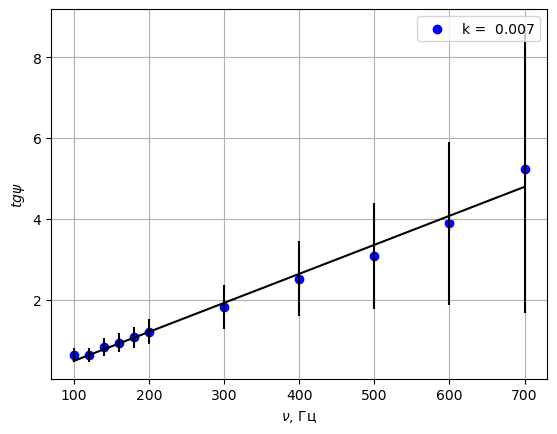
\includegraphics[width=13cm]{images/plot2.png}
    \caption{График зависимости фазового сдвига от частоты}
\end{figure}

\newpage
\begin{table}[h!]
    \centering
    \begin{tabular}{|c|c|c|c|}
        \hline
        $\nu$, Гц & $I$, мА & $U$, мВ & $\psi$, рад\\\hline
        1000  & 274.65 $\pm$ 0.05  & 643.2 $\pm$ 0.1 & 1.413 $\pm$ 0.314\\\hline
        1200  & 259.69 $\pm$ 0.05  & 610.9 $\pm$ 0.1 & 1.57  $\pm$ 0.314\\\hline
        1440  & 242.52 $\pm$ 0.05  & 570.7 $\pm$ 0.1 & 1.57  $\pm$ 0.314\\\hline
        1728  & 222.73 $\pm$ 0.05  & 523.7 $\pm$ 0.1 & 1.57  $\pm$ 0.314\\\hline
        2070  & 201.74 $\pm$ 0.05  & 472.9 $\pm$ 0.1 & 1.727 $\pm$ 0.314\\\hline
        2480  & 179.95 $\pm$ 0.05  & 419.3 $\pm$ 0.1 & 1.727 $\pm$ 0.314\\\hline
        2980  & 157.53 $\pm$ 0.05  & 364.6 $\pm$ 0.1 & 1.884 $\pm$ 0.314\\\hline
        3580  & 136.33 $\pm$ 0.05  & 311.8 $\pm$ 0.1 & 1.884 $\pm$ 0.314\\\hline
        4300  & 116.73 $\pm$ 0.05  & 262.6 $\pm$ 0.1 & 1.884 $\pm$ 0.314\\\hline
        5160  & 99.14  $\pm$ 0.05  & 218.0 $\pm$ 0.1 & 2.041 $\pm$ 0.314\\\hline
        6190  & 83.6   $\pm$ 0.05  & 178.2 $\pm$ 0.1 & 2.198 $\pm$ 0.314\\\hline
        7430  & 70.04  $\pm$ 0.05  & 143.2 $\pm$ 0.1 & 2.355 $\pm$ 0.314\\\hline
        8920  & 58.18  $\pm$ 0.05  & 112.7 $\pm$ 0.1 & 2.512 $\pm$ 0.314\\\hline
        10700 & 47.9   $\pm$ 0.05  & 87.1  $\pm$ 0.1 & 2.826 $\pm$ 0.314\\\hline
        12840 & 38.578 $\pm$ 0.005 & 65.3  $\pm$ 0.1 & 2.826 $\pm$ 0.314\\\hline
        15410 & 30.735 $\pm$ 0.005 & 48.6  $\pm$ 0.1 & 3.297 $\pm$ 0.314\\\hline
        18490 & 23.64  $\pm$ 0.005 & 36.0  $\pm$ 0.1 & 3.768 $\pm$ 0.314\\\hline
        22190 & 17.046 $\pm$ 0.005 & 27.2  $\pm$ 0.1 & 4.239 $\pm$ 0.314\\\hline
        26630 & 10.724 $\pm$ 0.005 & 20.7  $\pm$ 0.1 & 4.396 $\pm$ 0.314\\\hline
    \end{tabular}
    \caption{Показания вольтметра и амперметра при высоких частотах от $0.5\nu_h$ до $15\nu_h$}
\end{table}

\begin{figure}[h!]
    \centering 
    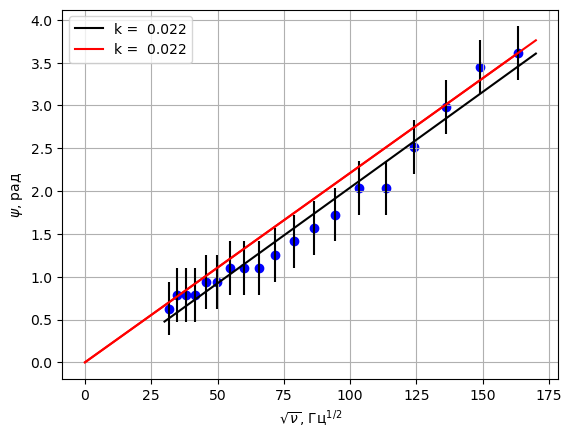
\includegraphics[width=12cm]{images/plot3.png}
    \caption{График зависимости фазового сдвига от квадрата частоты}
\end{figure}
\newpage 
\subsection*{Измерение индуктивности катушки}

\begin{figure}[h!]
    \begin{minipage}{0.5\linewidth}
        \centering
        \begin{tabular}{|c|c|c|}
            \hline
        $\nu$, Гц & $L$, мГн\\\hline
        50   & 9.88  $\pm$ 0.05\\\hline
        150  & 7.25  $\pm$ 0.05\\\hline
        250  & 5.36  $\pm$ 0.05\\\hline
        400  & 4.08  $\pm$ 0.05\\\hline
        500  & 3.69  $\pm$ 0.05\\\hline
        600  & 3.46  $\pm$ 0.05\\\hline
        800  & 3.21  $\pm$ 0.05\\\hline
        1500 & 2.97  $\pm$ 0.05\\\hline
        4000 & 2.89  $\pm$ 0.05\\\hline
        7500 & 2.92  $\pm$ 0.01\\\hline
        12000& 3.05  $\pm$ 0.01\\\hline
        16200& 3.31  $\pm$ 0.01\\\hline
        20000& 3.71  $\pm$ 0.01\\\hline
        \end{tabular}
    \captionof{table}{Зависимость индуктивности катушки от частоты}
    \end{minipage}
    \begin{minipage}{0.5\linewidth}
        \centering
        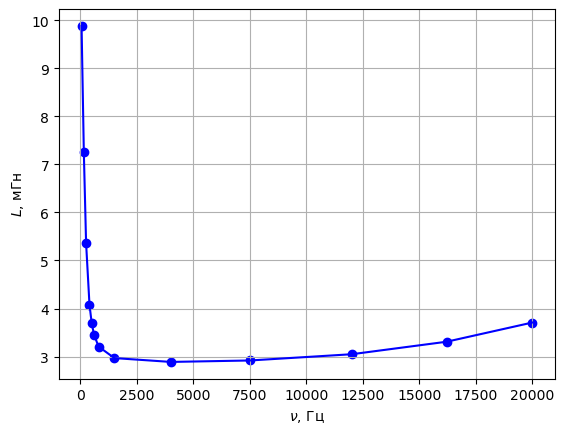
\includegraphics[width=10cm]{images/plot4.png}
        \captionof{figure}{Гарфик зависимости индуктивности от частоты}
    \end{minipage}
\end{figure}


